\documentclass[10pt, a4paper]{article}
\usepackage[paper=a4paper, left=1.5cm, right=1.5cm, bottom=1.5cm, top=3.5cm]{geometry}
\usepackage[latin1]{inputenc}
\usepackage[T1]{fontenc}
\usepackage[spanish]{babel}
\usepackage{indentfirst}
\usepackage{fancyhdr}
\usepackage{latexsym}
\usepackage{lastpage}
\usepackage{graphicx}
\usepackage{caption}
\usepackage{subfigure}
\usepackage{caratula}
\usepackage[colorlinks=true, linkcolor=blue]{hyperref}
\usepackage{calc}


\sloppy

\parskip=5pt % 10pt es el tama�o de fuente

% Pongo en 0 la distancia extra entre �temes.
\let\olditemize\itemize
\def\itemize{\olditemize\itemsep=0pt}

% Acomodo fancyhdr.
\pagestyle{fancy}
\thispagestyle{fancy}
\addtolength{\headheight}{1pt}
\lhead{Algoritmos y Estructuras de Datos III}
\rhead{$1^{\mathrm{er}}$ cuatrimestre de 2014}
\cfoot{\thepage /\pageref{LastPage}}
\renewcommand{\footrulewidth}{0.4pt}

\author{Algoritmos y Estructuras de Datos III, DC, UBA.}
\date{}
\title{Trabajo pr\'actico 1}

\begin{document}

\titulo{Trabajo Practico 1}
\submateria{Primer cuatrimestre 2014}
\materia{Algoritmos y Estructura de Datos III}
\grupo{Grupo 1}
\integrante{Blundi, Solange}{336/10}{solange.blundi@gmail.com}
\integrante{Paez, Ariel}{???/??}{twizt.hl@gmail.com}
\integrante{Guerson, Matias}{???/??}{matias.guerson@gmail.com}
\integrante{Inzaghi Pronesti, Patricio Ezequiel}{255/11}{pinzaghi@dc.uba.ar}
\maketitle

\newpage

\tableofcontents

\newpage
\section{Problema 1: Camiones sospechosos}
\subsection{Descripci\'on del problema}

En este ejercicio se nos presenta el juego Roban\'umeros, un juego de dos jugadores que consiste en lo siguiente:

\begin{itemize}
\item Se juega con cartas y cada una tiene un n\'umero entero
\item Se juega por turnos alternados entre ambos jugadores. Un jugador no puede elegir pasar, es decir que debe jugar en todos sus turnos
\item Al comenzar el juego se pone sobre la mesa una secuencia de cartas boca arriba, la cantidad puede ser cualquiera
\item En su turno el jugador puede tomar la cantidad de cartas que quiera. Las cartas tomadas deben ser adyacentes y el jugador puede elegir de qu\'e extremo sacarlas (izquierda o derecha). 
\item El juego termina cuando se terminan las cartas
\item Gana el jugador que sume m\'as puntos con las cartas que tom\'o
\end{itemize}

Un ejemplo de la disposici\'on inicial de las cartas puede ser el siguiente:\\

\begin{figure}[h]
\begin{center}

\includegraphics[scale=0.6]{./img/ej1_explicacion1.png}
\caption{Caso ejemplo}
\end{center}
\end{figure}

En este caso, un jugador podr\'ia robar las cartas 2, -4 y 6 o -10, 9, 1, 6, pero no 2, 6, 9 ya que no son adyacentes. \\

Para este caso en particular el juego se desarrollar\'ia de la siguiente manera:

\begin{itemize}
\item Mingo toma 5 cartas desde la izquierda (2, -4, 6, 1 y 9) sumando 14 puntos.
\item An\'ibal toma la \'unica carta restante, el -10.
\end{itemize}

El juego lo gana Mingo logrando una diferencia de 24 puntos.

\subsection{Resoluci\'on}

Para resolver el problema dado de $C$ cartas de longitud $n$, debemos construir una funcion $F$ tal que F(C[0..n-1]) est\'e definida como "La jugada que logre la mejor diferencia con el oponente, sabiendo que el mismo juega de forma \'optima" \\

Pensando de manera mas precisa la funci\'on, podriamos escribirla como: \\

F(C[0..n-1]) = MAX(Tomar una carta desde la izquierda y restarle F(C[1..n-1]), Tomar dos cartas desde la izquierda y restarle F(C[2..n-1]), ..., Tomar todas las cartas, ... , Tomar n-2 cartas desde la derecha y restarte F(C[0..0])) \\

Como podemos ver, habr\'ia que tomar la m\'axima diferencia de puntos obtenidos entre las cartas que uno toma y las que toma el oponente, que tambien juega de manera \'optima. La jugada del rival es evaluar la misma funci\'on para el resto de las cartas que dejamos. \\

Definamos esta funci\'on recursivamente (usamos una funci\'on $h$ para lograr claridad): \\

$
F(P) =
\left\{
	\begin{array}{ll}
		P_{0}  & \mbox{if } |P| = 1 \\
		max( h_{izq} (0, n), ... , h_{izq} (k, n) , ... , \sum\limits_{i=0}^n P_{i} , h_{der} (n-1, n), ... , h_{der} (k, n) , ... )  & \mbox{if } |P| > 1
	\end{array}
\right.
$ \\

Las funciones $h_{izq}$ y $h_{der}$ devuelven la diferencia de una jugada en particular tomando una cantidad de cartas y restandole el puntaje del rival con las cartas restantes: \\

$h_{izq}(fin, n) =  (\sum\limits_{i=0}^{fin} C_{i}) - F(C[fin+1...n-1])$ \\
$h_{der}(inicio, n) =  (\sum\limits_{i=inicio}^{n-1} C_{i}) - F(C[0...inicio-1])$\\

Podemos interpretar la funci\'on F como un arbol con todas las posibilidades y finalmente nos devuelve la mejor diferencia posible. Como podemos ver en el ejemplo esta clase de problemas tiene solapamiento de subsoluciones, por lo cual una versi\'on recursiva a secas no es la manera \'optima de implementar la soluci\'on. 

\begin{figure}[h]
\begin{center}
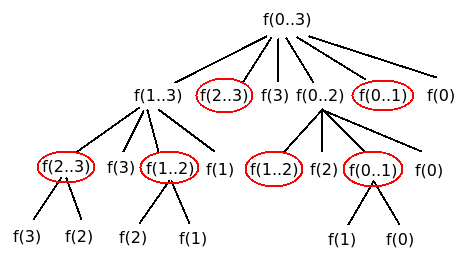
\includegraphics[scale=0.6]{./img/ej1_res1.png}
\caption{\'Arbol representativo de la funci\'on recursiva con los subproblemas requeridos para cada problema en particular, en rojo se marcan los subproblemas solapados}
\end{center}
\end{figure}

Notar que las hojas de este arbol son los casos base y no los consideramos casos repetidos ya que resolverlos tiene una complejidad O(1) como veremos mas adelante. \\

Para evitar volver a calcular subproblemas, decidimos guardar en una matriz de $n*n$ las distintas subsoluciones posibles y en otra tabla de igual tama\~no que combinaci\'on de cartas logr\'o ese resultado. Por ejemplo el subproblema (caso base) F(C[0..0]) est\'a representado por la fila 0 columna 0, pero el resultado al problema total F(C[0..5]) est\'a en la fila 0 columna 5.\\

Sabemos que el caso base de nuestro problema es cuando queda una sola carta. Como estamos obligados a levantar al menos una, es la \'unica opci\'on posible, con lo cual la diagonal de nuestra matriz queda determinada facilmente. 

\begin{figure}[h]
\begin{center}
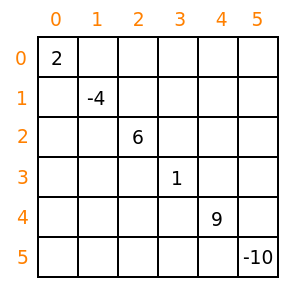
\includegraphics[scale=0.6]{./img/ej1_res2.png}
\caption{Tabla de resultados de F con el problema de ejemplo dado en la secci\'on "Descripci\'on del problema"}
\end{center}
\end{figure}

A partir de ese llenado inicial, podemos ir determinando el resto de los valores de la tabla. En general, un problema de rango $i$ a $j$ siempre usara subproblemas acotados entre estos valores, entonces para un determinado problema F(C[i..j]) alcanza con tener los valores de la tabla de la fila $i$ y de la columna $j$ hasta la posici\'on que estamos calculando.

\newpage

\begin{figure}[h]
\begin{center}
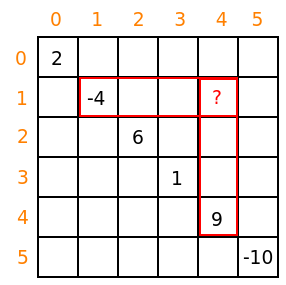
\includegraphics[scale=0.6]{./img/ej1_res3.png}
\caption{Casilleros requeridos para resolver el problema F(C[1..4])}
\end{center}
\end{figure}

Llenando la tabla de abajo hacia arriba y de izquierda a derecha garantiza que siempre tendremos los subproblemas necesarios para llenar el casillero actual. Por ejemplo, para calcular el problema F(C[3..5]) pondriamos en la fila 3 columna 5 el resultado de evaluar MAX(1-F(C[4..5]), 1+9 - F(C[5..5]), 1+9+(-10), -10 - F(C[3..4]), -10+9 - F(C[3..3])), como podemos ver en la tabla todos los subproblemas requeridos ya fueron calculados y sus valores los obtenemos en O(1) en esta ejecuci\'on.

\begin{figure}[h]
\begin{center}
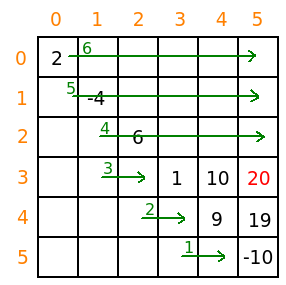
\includegraphics[scale=0.6]{./img/ej1_res4.png}
\caption{Orden de llenado}
\end{center}
\end{figure}

Al terminar de completar la tabla, tendremos el resultado del problema F(C[0..n]) en la fila 0 columna n.

\newpage
\subsection{Demostraci\'on del problema}

Vamos a demostrar el problema usando inducci\'on en la iteraci\'on del algoritmo que utilizamos. El pseudo codigo que nos interesa analizar es el siguiente:

\lstset{language=C++,
                basicstyle=\ttfamily\footnotesize,
                keywordstyle=\color{blue}\ttfamily,
                stringstyle=\color{red}\ttfamily,
                commentstyle=\color{green}\ttfamily,
                morecomment=[l][\color{magenta}]{\#},
                breaklines=true
}
\begin{lstlisting}
cartas_inicio = 0;

for(i = cant_cartas-1; i>=0; i--){

	for(int j = 0; j<cant_cartas; j++){
		
		q = 0
		
		if (i == j){
			q = CARTAS\_{i}
			cartas_inicio = i
		}else{
			q = SUM(CARTAS[cartas_inicio..j])
			
			for(k=cartas_inicio; k < j; k++)
				MAX(q, SUM(CARTAS[cartas_inicio][k]) - f[k+1][j])
			
			for(k=j; k > cartas_inicio; k--)
				MAX(q, SUM(CARTAS[k][j]) - f[cartas_inicio][k-1])
		}		
		
		f[i][j] = q
		
	}

}
\end{lstlisting}

\newpage 

\subsection{Complejidad del algoritmo}

Analizaremos la complejidad del algoritmo propuesto utilizando el siguiente pseudo c\'odigo como gu\'ia: \\

\begin{itemize}
\item crear una tabla de n*n, donde $n$ en es la cantidad de cartas. (Esto demora exactamente $n^2$ iteraciones)
\item para cada fila $f$ (Recorremos las n filas, $n$ iteraciones)
	\begin{itemize}
	\item para cada columna $c$ (Recorremos las n columnas, $n$ iteraciones)
		\begin{itemize}
			\item si es una casilla de la diagonal ($f = c$ caso base) (Esto se realiza en una operaci\'on)
				\begin{itemize}
				\item pongo en $tabla\_resultados(f,c)$ el valor de la carta C[f] (Esto se realiza en una operaci\'on)
				\end{itemize}
			\item si no es diagonal
				\begin{itemize}
				\item guardo en $x$ la suma de todas las cartas (Esto se hace en O(1) usando la tabla de sumas)
				\item guardo en $y$ el maximo valor de todas las combinaciones de tomar cartas desde la izquierda y restarles el puntaje \'optimo del oponente. (Son $n$ iteraciones de posibles subconjuntos de cartas donde se suman en O(1) y se les resta el resultado \'optimo en O(1), ambos datos sacados de la tablas)
				\item guardo en $z$ el maximo valor de todas las combinaciones de tomar cartas desde la derecha y restarles el puntaje \'optimo del oponente. (Son $n$ iteraciones de posibles subconjuntos de cartas donde se suman en O(1) y se les resta el resultado \'optimo en O(1), ambos datos sacados de la tablas)
				\item guardo en $tabla\_resultados(f,c)$ el $max(x,y,z)$ (Asignaci\'on en la tabla, O(1))
				\end{itemize}
		\end{itemize}
	\end{itemize}
\end{itemize}

Para lograr obtener la sumatoria de un rango de cartas en O(1) previamente cargamos una tabla con rangos de sumas de manera similar a la tabla que guarda los resultados de los problemas. Esto se realiza en $n^3$ una \'unica vez antes de comenzar a llenar la tabla de resultados. \\

Finalmente, nuestro algoritmo realiza $O(n^2 * 2*n)$ iteraciones, que es lo mismo que $O(n^2 * 2*n) = O(n^2*n) = O(n^3)$

\newpage

\subsection{C\'odigo fuente}

\lstset{language=C++,
                basicstyle=\ttfamily\footnotesize,
                keywordstyle=\color{blue}\ttfamily,
                stringstyle=\color{red}\ttfamily,
                commentstyle=\color{green}\ttfamily,
                morecomment=[l][\color{magenta}]{\#},
                breaklines=true
}
\begin{lstlisting}

// Lleno todas las posibles subcadenas de sumas en una tabla
for(int i = 0; i<cant_cartas; i++){
	for(int j = 0; j<cant_cartas; j++){
		(*tabla_sumatorias)[i][j] = sumatoria(cartas, i, j); 
	}
}
// Lleno la tabla con los resultados posibles
int cartas_inicio = 0;
int maxval = 0;

for(int i = cant_cartas-1; i>=0; i--){
	
	for(int j = 0; j<cant_cartas; j++){
		
		if(i<=j){
			
			int q = (int) -INFINITY;

			if(i==j){
				// Casos base, la mejor opcion es la unica carta que hay
				cartas_inicio = i;
				q = cartas[j];
				(*tabla_elecciones)[i][j] = pair<int,int>(0,1);
			}else{
				
				// Agarrar todas las cartas
				maxval = max(q, (*tabla_sumatorias)[cartas_inicio][j]);
				// Actualizo la mejor jugada encontrada hasta el momento
				if(maxval>q){
					(*tabla_elecciones)[i][j] = pair<int,int>(0,j-cartas_inicio+1);
				}
				q = maxval;
				
				// Agarrar desde la izquierda y restarle la jugada optima del rival
				for(int k=cartas_inicio; k < j; k++){
					maxval = max(q, (*tabla_sumatorias)[cartas_inicio][k] - (*tabla_resultados)[k+1][j]);
					// Actualizo la mejor jugada encontrada hasta el momento
					if(maxval>q){
						(*tabla_elecciones)[i][j] = pair<int,int>(0,k-cartas_inicio+1);
					}
					q = maxval;
				}
				
				// Agarrar desde la derecha y restarle la jugada optima del rival
				for(int k=j; k > cartas_inicio; k--){
					maxval = max(q, (*tabla_sumatorias)[k][j] - (*tabla_resultados)[cartas_inicio][k-1]);
					// Actualizo la mejor jugada encontrada hasta el momento
					if(maxval>q){
						(*tabla_elecciones)[i][j] = pair<int,int>(1,k-cartas_inicio+1);
					}
					q = maxval;
					
				}

			}
			// q = Max(sumatoria(cartas_{0,0}) - tabla_resultados_{1,n} , ... , sumatoria(cartas_{0,n}))
			(*tabla_resultados)[i][j] = q;
			
		}
		
	}
	
}


\end{lstlisting}

\newpage

\subsection{Casos de prueba}

Incorporamos entre los archivos adjuntos, en TP:/ej1/input/, varios casos de prueba, entre ellos algunos casos borde y otros triviales para comprobar la correctitud del algoritmo.

\begin{itemize}
\item Negativos Iguales: En este caso el juego es con un n\'umero par de cartas con el mismo n\'umero negativo. Como cada jugador juega \'optimamente, agarrar\'an s\'olo una carta por mano, y como hay una cantidad par de cartas, el juego termina con una diferencia 0 (cero) entre ambos jugadores.
\item Trivial: Consiste en un juego de cartas todas positivas, por lo que el primer jugador obtendr\'a la mayor diferencia agarrando todas las cartas.
\item TP: Es el ejemplo dado en el enunciado del TP, ejecutando el algoritmo con este input constatamos que la mayor diferencia jugando \'optimamente se obtiene cuando el primer jugador toma las primeras 5 cartas dejandole al segundo jugador solo la \'ultima, logrando una  diferencia de 24.   
\item Negativos: Es un juego de cartas con valores negativos, este caso en principio fu\'e pensado para constatar el correcto funcionamiento del algoritmo cuando las cartas solo tienen valores negativos . 
\item Simple: Consiste en una cantidad peque\~na de cartas, exactamente cuatro, donde una sola es negativa, para que el primer jugador no agarre todas y as\'i gane como en el input Trivial.
\end{itemize}

\newpage


\subsection{Performance}


\newpage
\section{Problema 2: La joya del Rio de la Plata}
\subsection{Descripci\'on del problema}

En este punto se nos pide resolver el problema de ubicar centrales de gas de manera estrat\'egica entre los pueblos de una cierta regi\'on.\\

Dados $n$ pueblos con sus respectivas coordenadas en el plano y $k$ centrales de gas, la idea es decidir en qu\'e pueblos ubicar las centrales. Adem\'as es posible construir tuber\'ias entre pueblos: una tuber\'ia que va de un pueblo con central a uno sin no s\'olo transporta el gas a este \'ultimo sino que adem\'as lo convierte en potencial proveedor. Es decir que se da una especie de transitividad entre los pueblos: si un pueblo $a$ con central de gas se conecta a otro pueblo $b$ y a su vez $b$ se conecta con $c$ entonces $c$ tambi\'en recibe gas (y puede distribuirlo).\\

El \'unico problema que presentan las tuber\'ias es que, a mayor longitud aumenta la posibilidad de rotura de las mismas. Evidentemente \'este es un factor que se quiere evitar, por lo cual se nos pide que, al elegir los pueblos donde instalar las centrales y y las conecciones entre los mismos minimicemos el tama\~no de la tuber\'ia m\'as larga.\\

Veamos algunos ejemplos, la siguiente es una situacion trivial en la que tenemos la misma cantidad de pueblos que de centrales:

\begin{figure}[h]
\begin{center}
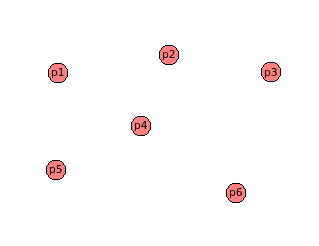
\includegraphics[scale=0.7]{./img/ej2_explicacion1.png}
\caption{Caso trivial}
\end{center}
\end{figure}

Los circulos colorados indican donde fueron instaladas las centrales, en este caso no hay ninguna tuber\'ia.\\

Veamos el siguiente caso mas complejo: 

\begin{figure}[h]
\begin{center}
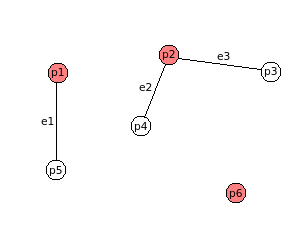
\includegraphics[scale=0.7]{./img/ej2_explicacion2.png}
\caption{Caso con K = 3 y N = 6}
\end{center}
\end{figure}

Como dato, sabemos que $e_2 < e_3 < e_1$ con lo cual nuestro largo m\'aximo de tuber\'ia es $e_1$

\subsection{Resoluci\'on}

Para la resoluci\'on del problema decidimos primero modelarlo con grafos, de forma que los nodos representen los pueblos, y las aristas (con pesos) las posibles conexiones entre pueblos. Los pesos est\'an dados por las distancias entre cada par de pueblos. \\

Como se nos pide minimizar el riesgo de rotura de las tuber\'ias a instalar, lo ideal ser\'ia lograr un esquema de conexiones tal que el largo de la tuber\'ia mas larga sea m\'inimo. Como veremos m\'as adelante, la ubicaci\'on de las centrales de gas no es de gran importancia ya que la transimisi\'on del servicio de gas se da por transitividad entre pueblos conectados (mientras alguno de ellos tenga una central). Por lo tanto lo importante es tener grupos de pueblos conectados a una misma central de manera que las tuber\'as necesarias sean de tama\~no m\'inimo. \\

Para obtener el esquema de conexiones antes mencionado partimos de pensar la regi\'on como un grafo completo; es decir que suponemos que todas las ciudades est\'an conectadas entre s\'i. Luego, a partir del grafo completo la idea es obtener un \'arbol generador m\'inimo del mismo utilizando el algoritmo de Prim.\\
Finalmente cortamos las $k - 1$ aristas m\'as largas del \'arbol, obteniendo un grafo de $k$ componentes conexas tal que la arista m\'as larga del grafo es de peso m\'inimo.\\ 
Como se dijo antes, es indistinto cu\'al de los pueblos de cada componente conexa tiene instalada la central. Sin embargo, como el ejercicio pide especificar el pueblo elegido, instalamos inicialmente una central en la ra\'iz del \'arbol. Luego, por cada arista ($v_1$, $v_2$) que eliminamos instalamos una central en el pueblo representado por $v_2$. %TODO: aclarar por que anda

\subsubsection{Implementaci\'on de Prim}
Describimos a continuaci\'on nuestra implementaci\'on del algoritmo de Prim.\\

Elegimos como ra\'iz del \'arbol generador m\'inimo al primer pueblo de la lista de pueblos de la regi\'on. Como al menos va a haber una central, instalamos una en el pueblo ra\'iz.\\
Luego realizamos un ciclo que se repite $n - 1$ veces (siendo $n$ la cantidad de nodos, es decir, ciudades), en el cual en cada iteraci\'on obtenemos el nodo m\'as cercano al \'arbol y lo agregamos al mismo.\\
Para saber cu\'al es el nodo m\'as cercano al \'arbol debemos, en cada iteraci\'on calcular la distancia m\'inima entre cada nodo que no pertenece al \'arbol y los que s\'i pertenecen.\\
Como partimos de un \'arbol que s\'olo tiene al primer nodo de la lista ($n_0$) inicialmente calculamos la distancia de cada uno de los nodos restantes a $n_0$. Luego se elegimos el nodo de menor distancia y lo agregamos al \'arbol y repetimos el proceso de calcular distancias y elegir el nodo m\'as cercano.\\
As\'i ,cada vez que agregamos un nodo al \'arbol volvemos a computar la m\'inima distancia de los nodos restantes comparando la distancia que cada uno tiene guardada como m\'inima con la distancia al nuevo nodo.\\
Una vez agregados todos los nodos al \'arbol tenemos un \'arbol generador m\'inimo.\\

\subsection{Demostraci\'on de la resoluci\'on}

\subsection{Complejidad del algoritmo}

Veamos la complejidad del algoritmo propuesto utilizando un pseudoc\'odigo que facilite el an\'alisis.

\begin{itemize}
\item poner puebloNuevo $\leftarrow$ primer pueblo de la lista
\item agregar a arbolPueblos $\leftarrow$ (puebloNuevo, puebloNuevo)
\item instalar central en puebloNuevo y poner centralesInstaladas $\leftarrow$ 1
\item poner i $\leftarrow$ 0
\item mientras i < cantidadPueblos - 1 (Agregamos los pueblos uno a uno, n iteraciones)
\begin{itemize}
	\item actualizarDistancias respecto a puebloNuevo (Lo analizamos m\'as adelante, toma O(n))
	\item poner masCercano $\leftarrow$ pueblo mas cercano fuera del arbol
	\item poner cercanoEnArbol $\leftarrow$ pueblo del arbol con el que masCercano tiene distancia minima
	\item agregar arbolPueblos $\leftarrow$ (cercanoEnArbol, masCercano) (Agregar un elemento a una lista es O(1))
\end{itemize}
\item ordenar arbolPueblos de mayor a menor por distancia entre pares 
\item mientras centralesInstaladas < cantidadCentralitas (k iteraciones, que a lo sumo son n)
\begin{itemize}
	\item poner aristaMayor $\leftarrow$ primer elem de arbolPueblos
	\item instalarCentral(aristaMayor.segundo)
	\item eliminar aristaMayor de arbolPueblos (eliminar usando erase es O(1))
\end{itemize}
\end{itemize}

Como se puede ver, la complejidad est\'a dada por el primer ciclo, el cual hace n iteraciones (donde n corresponde a la cantidad de ciudades), ya que debe agregarlas una a una al \'arbol generador m\'inimo. Dentro de ese ciclo se actualizan las distancias de las ciudades al \'arbol; veremos la complejidad de hacerlo a continuaci\'on, pero podemos adelantar que realiza n iteraciones tambi\'en. Con lo cual la complejidad total del ciclo quedar\'ia en O(n).\\
Una vez obtenido el \'arbol lo ordenamos de mayor a menor, donde el par ($v_1$, $v_2$) es mayor a otro ($w_1$, $w_2$) si la distancia entre $v_1$ y $v_2$ es mayor a la distancia entre $w_1$ y $w_2$. Ordenar una lista con std::list::sort toma O(n*log(n)). \cite{sort}\\
Finalmente eliminamos los primeros k-1 (donde k es el n\'umero de centrales) pares de pueblos; es decir los pares que tienen mayor distancia. Cada eliminaci\'on toma O(1) usando std::list::erase \cite{erase}. En total toma O(k), que es a lo sumo O(n).\\

Vemos ahora el pseudoc\'odigo de actualizarDsitancias para confirmar que es O(n).\\

\begin{itemize}
\item poner puebloNuevo.distanciaAlArbol $\leftarrow$ 0
\item para cada pueblo en pueblos (iteramos todos los pueblos, O(n))
\begin{itemize}
	\item poner distanciaActual $\leftarrow$ pueblo.distanciaAlArbol
	\item si distanciaActual es mayor a 0 (el pueblo no es parte del arbol)
	\begin{itemize}
		\item poner distanciaNueva $\leftarrow$ distancia(puebloNuevo, pueblo)
		\item si distanciaNueva > distanciaActual poner pueblo.distanciaAlArbol $\leftarrow$ distanciaNueva
	\end{itemize}
\end{itemize}
\end{itemize}

En actualizarDistancias es claro que la complejidad est\'a dada por la iteraci\'on a trav\'es de las ciudades, es decir O(n). Luego, dentro del ciclo s\'olo se realizan comparaciones y asignaciones, que no afectan la complejidad significativamente.\\

Podemos decir ahora que la complejidad del algoritmo est\'a dada por el ciclo en el que se agregan nodos al \'arbol y que la misma es O($n^2$).

\newpage

\subsection{C\'odigo fuente}

\lstset{language=C++,
                basicstyle=\ttfamily\footnotesize,
                keywordstyle=\color{blue}\ttfamily,
                stringstyle=\color{red}\ttfamily,
                commentstyle=\color{green}\ttfamily,
                morecomment=[l][\color{magenta}]{\#},
                breaklines=true
}
\begin{lstlisting}

/* Constructor de region */
Region::Region(list<Pueblo*> * lista_pueblos, int centralitas){
	
	_centralitas = centralitas;
	_centrales_instaladas = 0;
	_tuberias_instaladas = 0;
	_pueblos = lista_pueblos;
	_arbol_pueblos = new list<pair<Pueblo*, Pueblo*> >();

}

void Region::resolver(){

	int cantPueblos = _pueblos->size();
	
	// Uso Prim para agregar pueblos al arbol

	// Elijo la primera ciudad de la lista como root
	Pueblo* puebloNuevo = *_pueblos->begin();
	pair<Pueblo*, Pueblo*> parPueblos = pair<Pueblo*, Pueblo*>(puebloNuevo, puebloNuevo);
	_arbol_pueblos->push_back(parPueblos);
	// Inicialmente solo el pueblo root tiene una central instalada
	puebloNuevo->instalarCentral();
	_centrales_instaladas = 1;

	// Pueblo mas cercano actual
	Pueblo * masCercano = puebloNuevo;

	// Agrego ciudades al arbol de a una - O(n)
	for(int i=0; i<cantPueblos-1 ; i++){
		
		// Actualizo las distancias al arbol y me quedo con la menor
		//cout << "nuevo_id: " << puebloNuevo->getId() << endl;
		masCercano = actualizarDistancias(puebloNuevo);

		// Agrego masCercano al arbol
		// En la proxima iteracion la distancia va a quedar en 0
		parPueblos = pair<Pueblo*, Pueblo*>(masCercano->getPuebloCercano(), masCercano);
		_arbol_pueblos->push_back(parPueblos);
		puebloNuevo = masCercano;
	}

	// Ordeno los pares de ciudades segun distancia (de mayor a menor)
	_arbol_pueblos->sort(compararDistancia);

	// Mientras que pueda instalar centrales achico el tam maximo de las tuberias
	// Es decir, genero k componentes conexas, cada una con una central

	list<pair<Pueblo*,Pueblo*> >::iterator p = _arbol_pueblos->begin();
	while (p != _arbol_pueblos->end()){
		if(_centrales_instaladas<_centralitas){
			// p representa la tuberia mas larga, la elimino e instalo una nueva central
			if(!((*p).second)->tieneCentral()){
				((*p).second)->instalarCentral();
				_centrales_instaladas+=1;
			}
			p = _arbol_pueblos->erase(p);
			
		}else{
			p++;
		}
	}
}

// Actualiza distancia minima al arbol de cada pueblo y devuelve el mas cercano
Pueblo* Region::actualizarDistancias(Pueblo* puebloNuevo){

	double distActual;
	double distNueva;
	double min = std::numeric_limits<double>::infinity();
	Pueblo* masCercano = puebloNuevo;

	// Antes de empezar actualizo la distancia del nuevo pueblo
	puebloNuevo->setDistanciaArbol(0.0);

	// Recorro todos los pueblos y actualizo sus distancias al arbol comparando con el ultimo p agregado
	for(list<Pueblo*>::iterator p = _pueblos->begin(); p != _pueblos->end(); p++){

		distActual = (**p).getDistanciaArbol();

		// Si no pertenece al arbol actualizo
		if(distActual > 0.0){

			distNueva = (**p).distancia(*puebloNuevo);
			
			if(distNueva < distActual){
				(**p).setPuebloCercano(puebloNuevo);
				(**p).setDistanciaArbol(distNueva);
			}

			distActual = (**p).getDistanciaArbol();

			// Si es el menor hasta el momento guardo la ciudad
			if(distActual < min){
				masCercano = *p;
			}
		}
	
	}

	return masCercano;
}

\end{lstlisting}

\subsection{Casos de prueba}

Como casos de prueba para el algoritmo elegimos inputs de los siguientes tipos:
\begin{itemize}
\item Casos en los que la cantidad de pueblos es igual a la cantidad de centrales.
\item Casos en los que la cantidad de pueblos es menor a la cantidad de centrales.
\end{itemize}

\subsection{Performance}

Para el an\'alisis de performance de este ejercicio decidimos ejecutar lotes aleatorios de tests siguiendo los siguientes criterios:

\begin{itemize}
	\item Iteramos entre 50.000 y alrededor de 80.000 pueblos.
	\item En cada iteraci\'on incrementamos la cantidad de pueblos en 1.000 unidades.
	\item Generamos un input con coordenadas aleatorias de los pueblos.
	\item Para cada iteraci\'on tomamos los siguientes valores de centrales:
	\begin{itemize}
		\item Comenzamos desde 1 central hasta 100.000.
		\item Incrementamos en cada iteraci\'on la cantidad de centrales en 4.000 unidades
	\end{itemize}
\end{itemize}

Para realizar esto generamos dos scripts de bash, uno que va iterando la cantidad de pueblos y centrales y por cada caso invoca al otro script, quien se encarga de generar las coordenadas aleatorias para la cantidad de pueblos deseada.

En cuanto a las cantidades de pueblos y centrales entendimos que para evitar la aleatoriedad en los resultados deb\'iamos ejecutar una gran cantidad de casos e ir incrementando la cantidad de pueblos hasta un n\'umero considerable. 
Adem\'as, nos pareci\'o interesante pasar por distintas cantidades de centrales, empezando por una, en la cual no iban a ser necesarios recortes de conexiones entre pueblos, e ir incrementando los valores hasta llegar a cantidades similares a la de pueblos, en donde iba a ser conveniente realizar m\'as recortes por ende la implementaci\'on iba a tener que realizar m\'as procesamiento y poder visualizar as\'i que la complejidad no se ve\'ia afectada.

\begin{center}
\begin{figure}[h!]
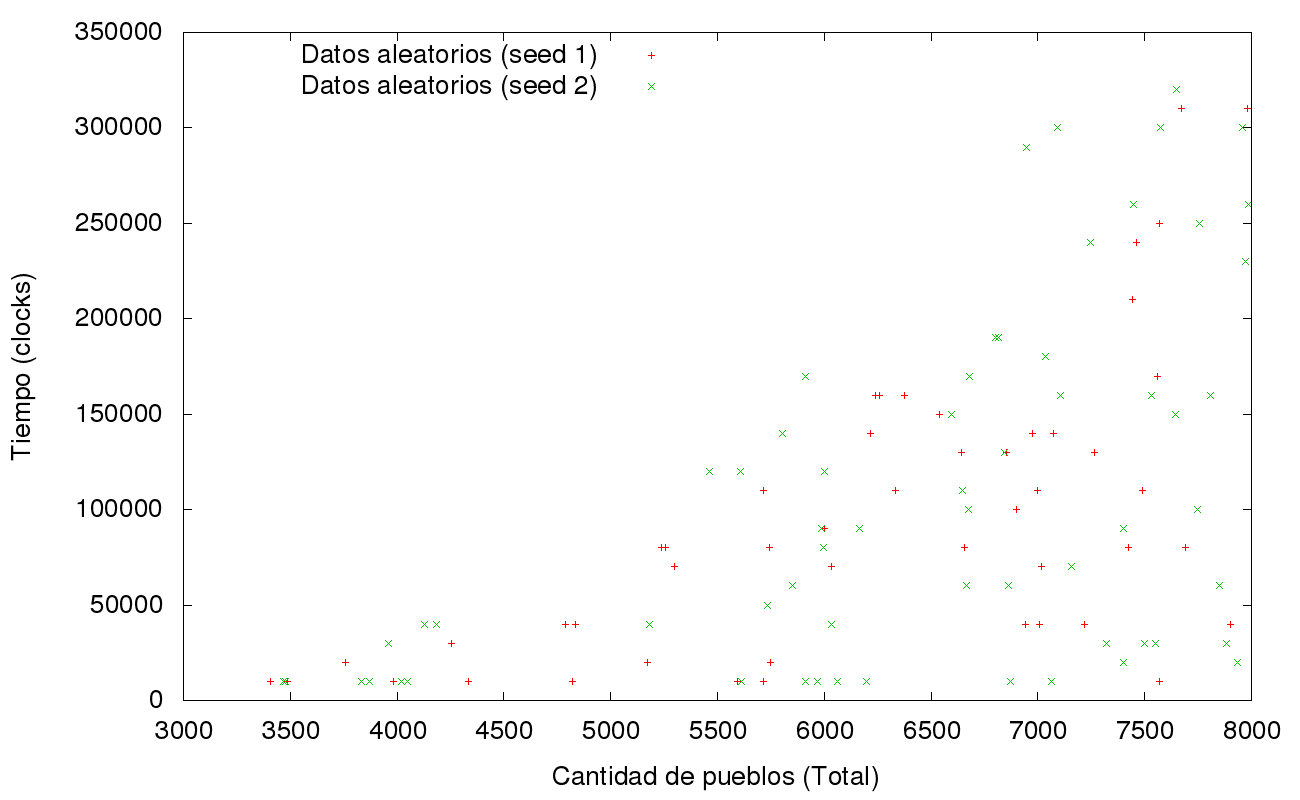
\includegraphics[scale=0.4]{./img/ej2_chart.png}
\caption{Tiempo transcurrido por cantidad de pueblos}
\end{figure}
\end{center}





Como podemos observar, con los datos obtenidos de las ejecuciones, se genera un gr\'afico con, a priori, la pinta de una funci\'on cuadr\'atica. 

Para poder observar este comportamiento mejor es necesario acompanarlo por la funci\'on $c*n*n$ con $c$ constante tal que permita ajustar la funci\'on cuadr\'atica al gr\'afico generado.

Para poder obtener dicha constante multiplicamos cada $n$, cantidad de pueblos, por si mismo y luego dividimos el tiempo resultante por dicho valor. De esta manera obtenemos una relaci\'on entre el cuadrado de la cantidad de pueblos y el tiempo de ejecuci\'on para cada valor. 
Finalmente, tomando un valor de $c$ apenas m\'as grande que el mayor obtenido en las anteriores operaciones, podemos aproximarnos a una constante que nos permita visualizar con mayor claridad que la complejidad solicitada no es superada y que el comportamiento se asemeja al deseado/solicitado.

Como peque\~na aclaraci\'on vale decir que los saltos que se producen en el eje x en el gr\'afico se corresponden con que ibamos iterando la cantidad de pueblos de mil en mil y es por eso que no se observan valores intermedios. 
As\'i tambi\'en, podemos observar que los distintos valores de tiempo para una misma cantidad de pueblos se corresponden con resultados para distintas cantidades de centrales.

Siguiendo por esta l\'inea de an\'alisis, entre los 55.000 y los 65.000 pueblos se puede notar una gran densidad en los valores, indicandonos que para dichas cantidades de pueblos, los tiempos de ejecuci\'on no se ven afectados por la cantidad de centrales.


\newpage
\section{Problema 3: Rompecolores}
\subsection{Descripci\'on del problema}

En este ejercicio se nos presenta el juego Saltos en la Matrix, el mismo se basa en el siguiente reglamento:

\begin{itemize}
\item Se posee un campo de juego cuadrado de N x N celdas.
\item Cada participante comienza en una posici\'on arbitraria $origen$ y debe llegar a la posici\'on $destino$.
\item Para moverse los participantes deber\'an ir saltando por las celdas de manera horizantal o vertical, no as\'i en diagonal.
\item Cada celda posee una potencia $p_{max}$ m\'axima de salto, los participantes podr\'an elegir una potencia $p$ entre 1 y $p_{max}$ para saltar hacia otra celda.
\item A modo de 'bonus' cada jugador posee $k$ unidades extra que podr\'a ir distribuyendo de la manera que desee y las mismas tienen como objetivo otorgarle a los participantes la posiblidad de realizar un salto m\'as potente de lo que la celda le proporciona en caso de creerlo conveniente. Por ejemplo, si un jugador est\'a ubicado en una celda que le posibilita saltar como mucho 2 celdas, pero el mismo considera beneficioso saltar 5, entonces el participante podr\'a utilizar 3 de sus unidades extra para realizar el salto deseado.
\end{itemize}

Como objetivo del ejercicio se nos pide presentar un algoritmo que tome los datos necesarios y devuelva como resultado una secuencia de saltos v\'alida que resuelva el problema en la menor cantidad de saltos posible.

Por otro lado el algoritmo no podr\'a tener una complejidad temporal de peor caso mayor a O($n^3 \cdot k$).

En caso de existir m\'as de una soluci\'on \'optima se podr\'a retornar cualquiera de ellas.


\subsection{Resoluci\'on y demostraci\'on}

Para la resoluci\'on del ejercicio decidimos modelar el tablero con un grafo dirigido. Una primera intuici\'on nos llev\'o a asignarle a cada casilla un nodo del grafo y las aristas que parten desde cada nodo representaban los posibles saltos entre casillas. Aunque este enfoque no es del todo incorrecto, no modela correctamente la variable de potencia adicional $k$ que uno posee a lo largo del juego. Si bien uno en una casilla de poder $p$ puede alcanzar las casillas tanto horizontales como verticales a distancia menor o igual a $p$, uno puede aumentar el rango de salto usando la potencia extra $k$. \\

Para poder representar esta informaci\'on en el grafo decidimos que los nodos ademas de representar casillas, representan a las mismas pero en distintos posibles estados. Estos estados pueden ser el no haber gastado ningun $k$ en el momento que se encuentra en esa casilla, o caso contrario cuanto fue gastado para llegar hasta esa casilla a lo largo del camino realizado.

\begin{figure}[h]
\begin{center}
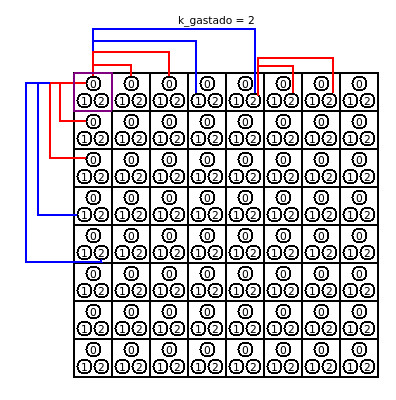
\includegraphics[scale=0.6]{./img/ej3_res1.png}
\caption{Ejemplo de modelado del grafo. Cada casilla posee k+1 nodos que representan sus posibles estados. En este ejemplo el k = 2 y el poder de salto de la casilla (1,1) marcada en violeta es p = 2. Las lineas rojas representan saltos sin usar unidades extra de potencia y las lineas azules usandolas.}
\end{center}
\end{figure}

Si unimos adecuadamente los nodos respetando las condiciones del juego, podremos modelar correctamente el tablero con todas sus condiciones. Luego solo restar\'a buscar el camino m\'inimo entre el nodo que represente la casilla de inicio y alguno de los nodos posibles de la casilla de salida. Las condiciones a respetar son las siguientes:

\begin{itemize}
\item Desde cualquier nodo (en cualquier estado $q$ de gasto de potencias extras) uno puede saltar hasta $p$ casilleros para cualquiera de los cuatro sentidos cardinales. Por ejemplo, desde la casilla (3,6) con poder de salto 2 en un tablero de 7x7, puedo llegar hasta las casillas (3,7), (3,5) y (3,4) horizontalmente y (1,6), (2,6), (4,6) y (5,6) verticalmente. Esto hace que nuestro algoritmo cree una arista entre los nodos que representan la casilla (3,6) y todos los nodos de las casillas que mencionamos anteriormente que representen el mismo estado $q$ de la casilla de origen.
\item Desde cualquier nodo en un estado $q$ de gasto de potencias extras y siendo $k$ el m\'aximo gasto extra posible, puedo saltar $p+(k-q)$ casilleros horizontal y verticalmente. Si el salto que realice supera los $p$ casilleros, el nodo de llegada debe ser el del casillero destino pero en estado igual a $q+k\_gastado$, donde $k\_gastado$ es el poder adicional usado para llegar a esa casilla. Esto garantiza tener una "memoria" de los $k$ utilizados durante uno de los caminos posibles. Notese que en los nodos que representan casillas con $k$ agotados, las unicas aristas posibles son las que solo utilizan la potencia de la casilla y siempre van a nodos que representan casillas sin $k$ restante. No hacer esto haria que el jugador gane unidades de $k$ que no le corresponden.
\end{itemize}

Una vez armado este grafo dirigido que contiene todos los posibles caminos desde todas las casillas (respetando las reglas del juego), solo resta ver cual es el camino con menor cantidad de saltos que logra llegar a la casilla de salida. Cabe destacar que nuestro grafo no es un grafo con pesos, ya que eliminamos ese factor creando aristas con todos los posibles caminos dependiendo el $p$ de la casilla. Este camino minimo lo buscamos con el algoritmo de recorrido de grafos BFS, una de sus utilidades es buscar caminos minimos en grafos sin peso o con todos pesos iguales.

\newpage
\subsection{Complejidad del algoritmo}

Analizaremos la complejidad del algoritmo propuesto utilizando el siguiente pseudo c\'odigo como gu\'ia:

\begin{itemize}
\item crear una tabla de n*n con las potencias de las casillas, donde $n$ en es el ancho/alto del tablero. (Esto demora exactamente $n^2$ iteraciones)
\item crear un grafo dirigido $G$ de n*n*(k+1) nodos. (Usamos un arreglo de listas enlazadas para representar el grafo. Crear el arreglo cuesta $n^2*(k+1)$ iteraciones, creando una lista vacia en cada iteraci\'on en tiempo constante.)
\item para cada nodo $v$ del grafo $G$ (Recorremos los nodos en $n^2*(k+1)$ iteraciones)
	\begin{itemize}
	\item para cada casilla $c$ de la fila del tablero donde se encuentra $v$ (Recorremos las n columnas del tablero, $n$ iteraciones)
		\begin{itemize}
			\item determino si debo unir el nodo $v$ con algun nodo de la casilla $c$ (Esto se realiza en tiempo constante ya que realiza operaciones matematicas y en caso de tener que unirlos agrega un elemento a una lista en tiempo constante)
		\end{itemize}
	\end{itemize}
	\begin{itemize}
	\item para cada casilla $c$ de la columna del tablero donde se encuentra $v$ (Recorremos las n filas del tablero, $n$ iteraciones)
		\begin{itemize}
			\item determino si debo unir el nodo $v$ con algun nodo de la casilla $c$ (Esto se realiza en tiempo constante ya que realiza operaciones matematicas y en caso de tener que unirlos agrega un elemento a una lista en tiempo constante)
		\end{itemize}
	\end{itemize}
\item busco el camino m\'inimo entre la casilla $inicio$ y la casilla $fin$ del grafo $G$ usando BFS ($O(n^3*k)$ (*))
\end{itemize}

(*) El algoritmo BFS tiene una complejidad de O(|V|+|E|), suponiendo el tablero mas denso posible donde se puede ir de cualquier casilla a cualquier casilla (de la misma fila o columna) tenemos $n^2*(k+1)$ nodos y $2*n$ aristas desde cada nodo, resultando $n^3*(k+1)$ aristas. |E| supera a |V| quedando una complejidad de $O(n^3*k)$ \\

Como analizamos, el algoritmo que asigna las aristas de cada uno de los $O(n^2*k)$ nodos se genera con un ciclo que anida 2 ciclos en paralelo de $n$ elementos, completandose toda esta operaci\'on en $O(n^2*k*2*n) = O(n^3*k)$. Finalmente se busca el camino m\'inimo en una complejidad del mismo orden de magnitud.

\newpage
\subsection{C\'odigo fuente}

\lstset{language=C++,
                basicstyle=\ttfamily\footnotesize,
                keywordstyle=\color{blue}\ttfamily,
                stringstyle=\color{red}\ttfamily,
                commentstyle=\color{green}\ttfamily,
                morecomment=[l][\color{magenta}]{\#},
                breaklines=true
}
\begin{lstlisting}
/*
 * Esta funcion decide dados dos nodos si hay una arista entre ellos y de que estado a que estado.
 * Si la hay, agrega la arista al grafo
*/
void unirNodos(directed_graph * grafo, int nro_nodo_fuente, int columna_nodo_fuente, int fila_nodo_fuente, int potencia_nodo_fuente, int estado_nodo_fuente, int columna_nodo_destino, int fila_nodo_destino, bool mirarFila, int tablero_casillas_por_lado, int tablero_k_inicial){
	
	int k_restantes = tablero_k_inicial-estado_nodo_fuente;
	int indice_fuente = 0;
	int indice_destino = 0;
	int nro_nodo_destino = 0;
	
	// Ajustamos los indices que nos interesan segun si estoy recorriendo fila o columna
	if(mirarFila){
		indice_fuente = columna_nodo_fuente;
		indice_destino = columna_nodo_destino;
	}else{
		indice_fuente = fila_nodo_fuente;
		indice_destino = fila_nodo_destino;
	}
	
	// Evito conectar la casilla consigo misma
	if(columna_nodo_fuente != columna_nodo_destino || fila_nodo_fuente!=fila_nodo_destino){
		
		// Verifico si el nodo de destino es alcanzable con la potencia de la casilla actual
		if( ((int) indice_fuente-potencia_nodo_fuente) <= (int) indice_destino && indice_destino <= (indice_fuente+potencia_nodo_fuente)){
			nro_nodo_destino = getNumeroNodo(tablero_casillas_por_lado, tablero_k_inicial, fila_nodo_destino, columna_nodo_destino, estado_nodo_fuente);
			// Conecto el nodo de la casilla actual en estado_nodo_actual 0 con el nodo de la casilla 
			// alcanzable en estado_nodo_actual 0 ya que no gaste ningun k para llegar ahi
			grafo->add_edge(nro_nodo_fuente,nro_nodo_destino);
		
		// Veo si puedo llegar usando k
		}else{
			int diferencia = indice_fuente-(potencia_nodo_fuente+k_restantes);
			
			// Si el poder de la casilla mas los k restantes del estado me lo permiten
			if( diferencia <= (int) indice_destino && indice_destino <= (indice_fuente+potencia_nodo_fuente+k_restantes)){
				int cuanto_k_necesito = 0;
				
				if(indice_fuente <= (int) indice_destino){
					cuanto_k_necesito = indice_destino - potencia_nodo_fuente - indice_fuente;
				}else{
					cuanto_k_necesito = indice_fuente - potencia_nodo_fuente - indice_destino;
				}
				// Lo voy a juntar con el nodo que puedo llegar pero a un estado correspondiente
				nro_nodo_destino = getNumeroNodo(tablero_casillas_por_lado, tablero_k_inicial, fila_nodo_destino, columna_nodo_destino, estado_nodo_fuente+cuanto_k_necesito);
				// Conecto el nodo de la casilla actual en estado_nodo_actual 0 con el nodo de la casilla 
				// alcanzable a su estado_nodo_actual correspondiente segun el gasto de k
				grafo->add_edge(nro_nodo_fuente,nro_nodo_destino);
			}
			
		}
	}
}

\end{lstlisting}

\newpage

\lstset{language=C++,
                basicstyle=\ttfamily\footnotesize,
                keywordstyle=\color{blue}\ttfamily,
                stringstyle=\color{red}\ttfamily,
                commentstyle=\color{green}\ttfamily,
                morecomment=[l][\color{magenta}]{\#},
                breaklines=true
}
\begin{lstlisting}

/*
 * Funcion que dada una fila, una columna y un estado de consumo de k, devuelve el numero de nodo correspondiente
 */
unsigned int getNumeroNodo(unsigned int tablero_casilleros_lado, unsigned int tablero_k, unsigned int fila, unsigned int col, unsigned int estado){
	
	unsigned int nro_nodo = (fila*tablero_casilleros_lado*(tablero_k+1) + (col*(tablero_k+1)) + estado);
	assert(0 <= nro_nodo);
	assert(nro_nodo < tablero_casilleros_lado*tablero_casilleros_lado*(tablero_k+1));
					
	return nro_nodo;
}
/*****************************/
/* CODIGO PRINCIPAL DEL MAIN */
/*****************************/

directed_graph * grafo = new directed_graph(cant_nodos);
		
unsigned int fila_nodo_fuente;
unsigned int columna_nodo_fuente;
unsigned int estado_nodo_fuente;
unsigned int potencia_nodo_fuente;

// Asigno las posibles aristas, i = todos los posibles nodos que representan tanto casillas sin gastos de k como con algun gasto
for(unsigned int nro_nodo_fuente = 0; nro_nodo_fuente<cant_nodos; nro_nodo_fuente++){
	
	// Datos de la casilla fuente
	fila_nodo_fuente = (nro_nodo_fuente / (k+1)) / n;
	columna_nodo_fuente = ((nro_nodo_fuente / (k+1)) % n);
	estado_nodo_fuente = nro_nodo_fuente % (k+1);
	potencia_nodo_fuente = (*potencias)[fila_nodo_fuente][columna_nodo_fuente];
					
	// Recorro la fila y conecto la casilla con todas las alcanzables de la misma
	for(unsigned int columna_nodo_destino=0; columna_nodo_destino<n; columna_nodo_destino++){
		
		int fila_nodo_destino = fila_nodo_fuente;
		
		// Si corresponde, se unen el nodo_fuente con el nodo_destino
		unirNodos(grafo, nro_nodo_fuente, columna_nodo_fuente, fila_nodo_fuente, potencia_nodo_fuente, estado_nodo_fuente, columna_nodo_destino, fila_nodo_destino, true, n, k);

	}
	// Recorro la columna y conecto la casilla con todas las alcanzables de la misma
	for(unsigned int fila_nodo_destino=0; fila_nodo_destino<n; fila_nodo_destino++){
		
		int columna_nodo_destino = columna_nodo_fuente;
		
		// Si corresponde, se unen el nodo_fuente con el nodo_destino
		unirNodos(grafo, nro_nodo_fuente, columna_nodo_fuente, fila_nodo_fuente, potencia_nodo_fuente, estado_nodo_fuente, columna_nodo_destino, fila_nodo_destino, false, n, k);
		
	}
}

\end{lstlisting}

\newpage
\subsection{Casos de prueba}

\subsection{Performance}




\end{document}
